\documentclass[10pt]{article}
\advance\hoffset by -0.7 truein\relax


\usepackage{graphicx}
%\input{epsf}

\topmargin=-0.4in
%\leftmargin=-1in 
\textwidth=6.3in
\textheight=8.8in


\usepackage{amssymb}
\usepackage{latexsym}
\usepackage{amsmath}
\usepackage{enumerate}

\usepackage{hyperref}

\begin{document}

\title{{\huge{\bf{Sim.I.am: A Robot Simulator }}}\\
{{Coursera: Control of Mobile Robots}}}
\author{Jean-Pierre de la Croix}
\date{Last Updated: \today}

\maketitle
\tableofcontents
\newpage
\section{Introduction}
This manual is going to be your resource for using the simulator in the programming exercises for this course. It will be updated throughout the course, so make sure to check it on a regular basis. You can access it anytime from the course page on Coursera under \texttt{Programming Exercises}.

\subsection{Installation}

Download \texttt{simiam-coursera-week-X.zip} (where X is the corresponding week for the exercise) from the course page on Coursera under \texttt{Programming Exercises}. Make sure to download a new copy of the simulator \textbf{before} you start a new week's programming exercises, or whenever an announcement is made that a new version is available. It is important to stay up-to-date, since new versions may contain important bug fixes or features required for the programming exercises.

Unzip the \texttt{.zip} file to any directory.

\subsection{Requirements}

You will need a reasonably modern computer to run the robot simulator. While the simulator will run on hardware older than a Pentium 4, it will probably be a very slow experience. You will also need a copy of MATLAB. The simulator has been tested with MATLAB R2009a, so it is recommended that you use that version or higher. No additional toolboxes are needed to run the simulator.

\subsection{Bug Reporting}
If you run into a bug (issue) with the simulator, please leave a message in the discussion forums with a detailed description. The bug will get fixed and a new version of the simulator will be uploaded to the course page on Coursera.

\section{Mobile Robot}

The mobile robot platform you will be using in the programming exercises is the Khepera III (K3) mobile robot. The K3 is equipped with 11 infrared (IR) range sensors, of which nine are located in a ring around it and two are located on the underside of the robot. The IR sensors are complemented by a set of five ultrasonic sensors. The K3 has a two-wheel differential drive with a wheel encoder for each wheel. It is powered by a single battery on the underside and can be controlled via software on its embedded Linux computer.
\begin{figure}[h]
 \centering
 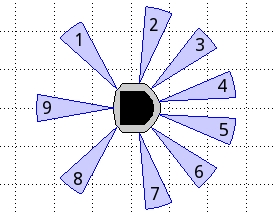
\includegraphics[bb=0 0 274 214,scale=0.6]{k3sensors.png}
 % k3sensors.png: 274x214 pixel, 72dpi, 9.66x7.55 cm, bb=0 0 274 214
 \caption{IR range sensor configuration}
 \label{fig:k3sensors}
\end{figure}




\subsection{IR Range Sensors}\label{irprox}
For the purpose of the programming exercises in the course, you will have access to the array of nine IR sensors that encompass the K3. IR range sensors are effective in the range $0.02$ m to $0.2$ m only. However, the IR sensors return raw values in the range of $[18,3960]$ instead of the measured distances. Figure \ref{fig:irvalues} demonstrates the function that maps these sensors values to distances.

\begin{figure}[h]
 \centering
 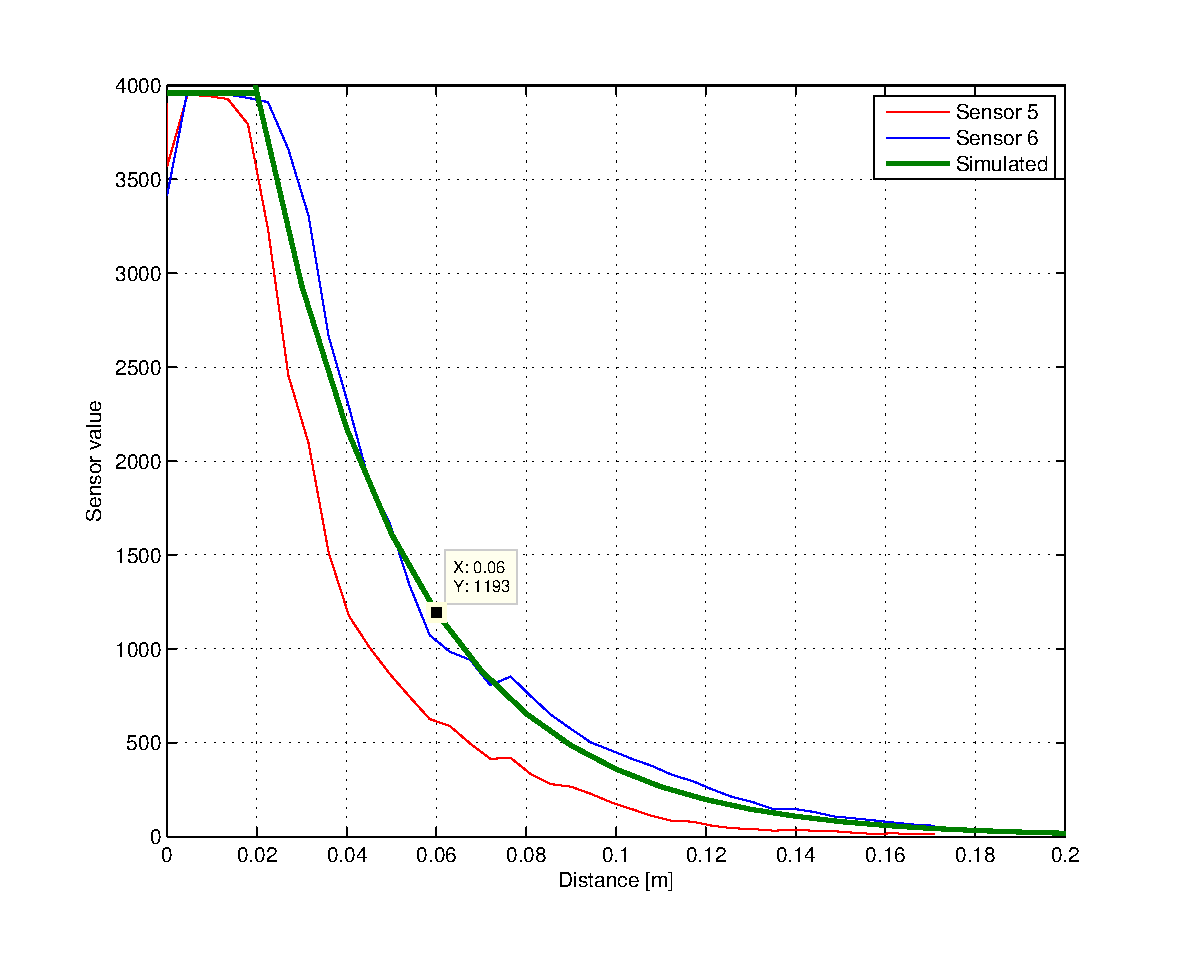
\includegraphics[scale=0.5]{./ir_actual.eps}
 % ir_actual.eps: 0x0 pixel, 300dpi, 0.00x0.00 cm, bb=   27   174   583   617
 \caption{Sensor values vs. Measured Distance}
 \label{fig:irvalues}
\end{figure}

The green plot represents the sensor model used in the simulator, while the blue and red plots show the sensor response of two different IR sensors (under different ambient lighting levels). The effect of ambient lighting (and other sources of noise) are \textbf{not} modelled in the simulator, but will be apparent on the actual hardware.

The function that maps distances, denoted by $\Delta$, to sensor values is the following piecewise function:
\begin{equation}
 f(\Delta) =
\begin{cases}
3960, & \text{if } 0\text{m} \leq \Delta \leq 0.02\text{m} \\
\lfloor3960e^{-30(\Delta-0.02)}\rfloor, & \text{if } 0.02\text{m} \leq \Delta \leq 0.2\text{m}
\end{cases}
\end{equation}

Your controller can access the IR array through the \texttt{robot} object that is passed into the \texttt{execute} function. For example,
\begin{verbatim}
 for i=1:9
    fprintf('IR #%d has a value of %d.\n', i, robot.ir_array(i).get_range());
 end
\end{verbatim}

The orientation (relative to the body of the K3, as shown in figure \ref{fig:k3sensors}) of IR sensors 1 through 9 is $128^\circ, 75^\circ, 42^\circ$, $13^\circ, -13^\circ, -42^\circ, -75^\circ, -128^\circ$, and $180^\circ$, respectively.

\subsection{Ultrasonic Range Sensors}
The ultrasonice range sensors have a sensing range of $0.2$m to $4$m, but are not available in the simulator.

\subsection{Differential Wheel Drive}\label{diffdrive}
Since the K3 has a differential wheel drive (i.e., is not a unicyle), it has to be controlled by specifying the angular velocities of the right and left wheel $(v_r,v_l)$, instead of the linear and angular velocities of a unicycle $(v,\omega)$. These velocities are computed by a transformation from $(v,\omega)$ to $(v_r,v_\ell)$. Recall that the dynamics of the unicycle are defined as,
\begin{equation}
 \begin{split}
   \dot{x} &= vcos(\theta) \\
   \dot{y} &= vsin(\theta) \\
   \dot{\theta} &= \omega.
 \end{split}
\end{equation}
The dynamics of the differential drive are defined as,
\begin{equation}
 \begin{split}
  \dot{x} &= \frac{R}{2}(v_r+v_\ell)cos(\theta) \\
  \dot{y} &= \frac{R}{2}(v_r+v_\ell)sin(\theta) \\
  \dot{\theta} &= \frac{R}{L}(v_r-v_\ell),
 \end{split}
\end{equation}
where $R$ is the radius of the wheels and $L$ is the distance between the wheels.

The speed of the K3 can be set in the following way assuming that you have implemented the \texttt{uni\_to\_diff} function, which transforms $(v,\omega)$ to $(v_r,v_\ell)$:
\begin{verbatim}
 v = 0.15; % m/s
 w = pi/4; % rad/s
 % Transform from v,w to v_r,v_l and set the speed of the robot
 [vel_r, vel_l] = obj.robot.dynamics.uni_to_diff(robot,v,w);
\end{verbatim}


\subsection{Wheel Encoders}
Each of the wheels is outfitted with a wheel encoder that increments or decrements a tick counter depending on whether the wheel is moving forward or backwards, respectively. Wheel encoders may be used to infer the relative pose of the robot. This inference is called \textbf{odometry}. The relevant information needed for odometry is the radius of the wheel, the distance between the wheels, and the number of ticks per revolution of the wheel. For example,

\begin{verbatim}
 R = robot.wheel_radius; % radius of the wheel
 L = robot.wheel_base_length; % distance between the wheels
 tpr = robot.encoders(1).ticks_per_rev; % ticks per revolution for the right wheel

 fprintf('The right wheel has a tick count of %d\n', robot.encoders(1).state);
 fprintf('The left wheel has a tick count of %d\n', robot.encoders(2).state);
\end{verbatim}

\section{Simulator}

Start the simulator with the \texttt{launch} command in MATLAB from the command window. It is important that this command is executed inside the unzipped folder (but not inside any of its subdirectories).

\begin{figure}[h]
 \centering
 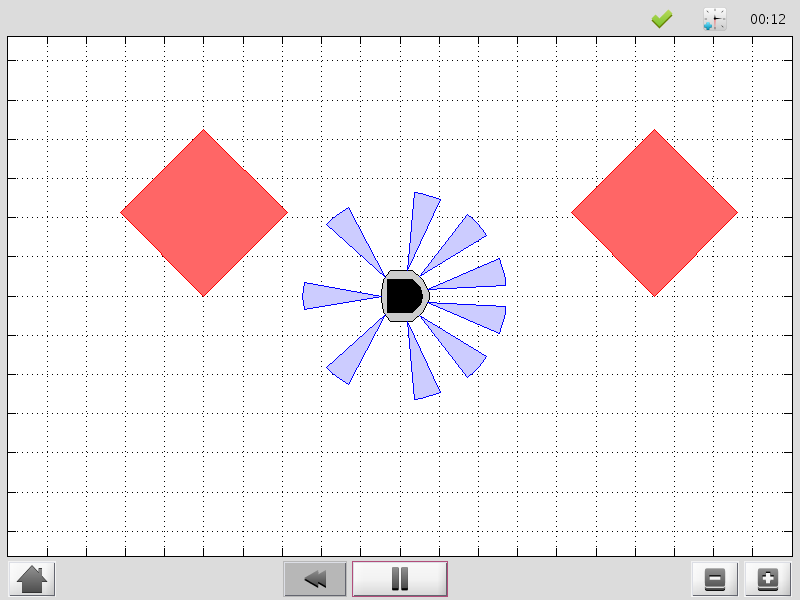
\includegraphics[scale=0.35]{simiam.png}
 \caption{Simulator}
 \label{fig:k3_sim}
\end{figure}

Figure \ref{fig:k3_sim} is a screenshot of the graphical user interface (GUI) of the simulator. The GUI can be controlled by the bottom row of buttons (or their equivalent keyboard shortcuts). The first button is the \textit{Home} button \texttt{[h]} and returns you to the home screen. The second button is the \textit{Rewind} button and resets the simulation. The third button is the \textit{Play} button \texttt{[p]}, which can be used to play and pause the simulation. The set of \textit{Zoom} buttons \texttt{[[,]]} or the mouse scroll wheel allows you to zoom in and out to get a better view of the simulation. The set of \textit{Pan} buttons \texttt{[left,right,up,down]} can be used to pan around the environment, or alternatively, Clicking, holding, and moving the mouse allows you to pan too. \textit{Track} button \texttt{[c]} can be used to toggle between a fixed camera view and a view that tracks the movement of the robot. You can also simply click on a robot to follow it.

\newpage
\section{Programming Exercises}

The following sections serve as a tutorial for getting through the simulator portions of the programming exercises. Places where you need to either edit or add code is marked off by a set of comments. For example,

\begin{verbatim}
  %% START CODE BLOCK %%
    [edit or add code here]
  %% END CODE BLOCK %%
\end{verbatim}

To start the simulator with the \texttt{launch} command from the command window, it is important that this command is executed inside the unzipped folder (but not inside any of its subdirectories).

\subsection{Week 1}

This week's exercises will help you learn about MATLAB and robot simulator:

\begin{enumerate}
\item Since the programming exercises involve programming in MATLAB, you should familiarize yourself with MATLAB and its language. Point your browser to \url{http://www.mathworks.com/academia/student_center/tutorials}, and watch the interactive MATLAB tutorial.

\item Familiarize yourself with the simulator by reading this manual and downloading the robot simulator posted on the ``Programming Exercises'' section on the Coursera page.
\end{enumerate}

\subsection{Week 2}
Start by downloading the robot simulator for this week from the ``Programming Exercises'' tab on Coursera course page. Before you can design and test controllers in the simulator, you will need to implement three components of the simulator:

\begin{enumerate}
 \item Implement the transformation from unicycle dynamics to differential drive dynamics, i.e. convert from $(v,\omega)$ to the right and left \textbf{angular} wheel speeds $(v_r,v_l)$.
 
 In the simulator, $(v,\omega)$ corresponds to the variables \texttt{v} and \texttt{w}, while $(v_r,v_l)$ correspond to the variables \texttt{vel\_r} and \texttt{vel\_l}. The function used by the controllers to convert from unicycle dynamics to differential drive dynamics is located in \texttt{+simiam/+robot/+dynamics/DifferentialDrive.m}. The function is named \texttt{uni\_to\_diff}, and inside of this function you will need to define \texttt{vel\_r} ($v_r$) and \texttt{vel\_l} ($v_l$) in terms of \texttt{v}, \texttt{w}, \texttt{R}, and \texttt{L}. \texttt{R} is the radius of a wheel, and \texttt{L} is the distance separating the two wheels. Make sure to refer to Section \ref{diffdrive} on ``Differential Wheel Drive'' for the dynamics.
 
 \item Implement odometry for the robot, such that as the robot moves around, its pose $(x,y,\theta)$ is estimated based on how far each of the wheels have turned. Assume that the robot starts at (0,0,0).
 
 The video lectures and, for example the tutorial located at \url{www.orcboard.org/wiki/images/1/1c/OdometryTutorial.pdf}, cover how odometry is computed. The general idea behind odometry is to use wheel encoders to measure the distance the wheels have turned over a small period of time, and use this information to approximate the change in pose of the robot.

 The pose of the robot is composed of its position $(x,y)$ and its orientation $\theta$ on a 2 dimensional plane (\textbf{note}: the video lecture may refer to robot's orientation as $\phi$). The currently estimated pose is stored in the variable \texttt{state\_estimate}, which bundles \texttt{x} ($x$), \texttt{y} ($y$), and \texttt{theta} ($\theta$). The robot updates the estimate of its pose by calling the \texttt{update\_odometry} function, which is located in \texttt{+simiam/+controller/+khepera3/K3Supervisor.m}. This function is called every \texttt{dt} seconds, where \texttt{dt} is $0.01$s (or a little more if the simulation is running slower).
 \begin{verbatim}  
  % Get wheel encoder ticks from the robot
  right_ticks = obj.robot.encoders(1).ticks;
  left_ticks = obj.robot.encoders(2).ticks;

  % Recall the wheel encoder ticks from the last estimate
  prev_right_ticks = obj.prev_ticks.right;
  prev_left_ticks = obj.prev_ticks.left;

  % Previous estimate 
  [x, y, theta] = obj.state_estimate.unpack();

  % Compute odometry here
  R = obj.robot.wheel_radius;
  L = obj.robot.wheel_base_length;
  m_per_tick = (2*pi*R)/obj.robot.encoders(1).ticks_per_rev;\end{verbatim}
  The above code is already provided so that you have all of the information needed to estimate the change in pose of the robot. \texttt{right\_ticks} and \texttt{left\_ticks} are the accumulated wheel encoder ticks of the right and left wheel. \texttt{prev\_right\_ticks} and \texttt{prev\_left\_ticks} are the wheel encoder ticks of the right and left wheel saved during the last call to \texttt{update\_odometry}. \texttt{R} is the radius of each wheel, and \texttt{L} is the distance separating the two wheels. \texttt{m\_per\_tick} is a constant that tells you how many meters a wheel covers with each tick of the wheel encoder. So, if you were to multiply \texttt{m\_per\_tick} by (\texttt{right\_ticks}-\texttt{prev\_right\_ticks}), you would get the distance travelled by the right wheel since the last estimate.
  
  Once you have computed the change in $(x,y,\theta)$ (let us denote the changes as \texttt{x\_dt}, \texttt{y\_dt}, and \texttt{theta\_dt}) , you need to update the estimate of the pose:
  \begin{verbatim}
    theta_new = theta + theta_d;
    x_new = x + x_dt;
    y_new = y + y_dt;\end{verbatim}
 
 \item Read the "IR Range Sensors" section in the manual and take note of the function $f(\Delta)$, which maps distances (in meters) to raw IR values. Implement code that converts raw IR values to distances (in meters).
 
 To retrieve the distances (in meters) measured by the IR proximity sensor, you will need to implement a conversion from the raw IR values to distances in the \texttt{get\_ir\_distances} function located in \texttt{+simiam/+robot/Khepera3.m}.
 \begin{verbatim}
  ir_distances = ir_array_values.*1;
  % OR
  ir_distances = zeros(1,9);
  for i = 1:9
      ir_distances(i) = ir_array_values(i)*1;
  end\end{verbatim}
  The variable \texttt{ir\_array\_values} is an array of the IR raw values. Section \ref{irprox} on ``IR Range Sensors'' defines a function $f(\Delta)$ that converts from distances to raw values. Find the inverse, so that raw values in the range $[18,3960]$ are converted to distances in the range $[0.02,0.2]$m. You can either do it by applying the conversion to the whole array (and thus apply it all at once), or using a \texttt{for} loop to convert each raw IR value individually. Pick one and comment the other one out.
 
 
\end{enumerate}

\subsubsection*{How to test it all}

To test your code, the simulator will is set to run a single P-regulator that will steer the robot to a particular angle (denoted $\theta_d$ or, in code, \texttt{theta\_d}). This P-regulator is implemented in \texttt{+simiam/+controller/} \texttt{GoToAngle.m}. If you want to change the linear velocity of the robot, or the angle to which it steers, edit the following two lines in \texttt{+simiam/+controller/+khepera3/K3Supervisor.m}
 \begin{verbatim}
  obj.theta_d = pi/4;
  obj.v = 0.1; %m/s\end{verbatim}
\begin{enumerate}
  \item To test the transformation from unicycle to differential drive, first set \texttt{obj.theta\_d=0}. The robot should drive straight forward. Now, set \texttt{obj.theta\_d} to positive or negative $\frac{\pi}{4}$. If positive, the robot should start off by turning to its left, if negative it should start off by turning to its left. \textbf{Note}: If you haven't implemented odometry yet, the robot will just keep on turning in that direction.
  \item To test the odometry, first make sure that the transformation from unicycle to differential drive works correctly. If so, set \texttt{obj.theta\_d} to some value, for example $\frac{\pi}{4}$, and the robot's P-regulator should steer the robot to that angle. You may also want to uncomment the \texttt{fprintf} statement in the \texttt{update\_odometry} function to print out the current estimate position to see if it make sense. Remember, the robot starts at $(x,y,\theta)=(0,0,0)$.
  \item To test the IR raw to distances conversion, edit \texttt{+simiam/+controller/}\texttt{GoToAngle.m} and uncomment the following section:
  \begin{verbatim}
  % for i=1:9
  %   fprintf('IR %d: %0.3fm\n', i, ir_distances(i));
  % end\end{verbatim}
  This \texttt{for} loop will print out the IR distances. If there are no obstacles (for example, walls) around the robot, these values should be close (if not equal to) $0.2$m. Once the robot gets within range of a wall, these values should decrease for some of the IR sensors (depending on which ones can sense the obstacle). \texttt{Note:} The robot will eventually collide with the wall, because we have not designed an obstacle avoidance controller yet!
\end{enumerate}


\subsection{Week 3}

Start by downloading the new robot simulator for this week from the ``Programming Exercises'' tab on the Coursera course page. This week you will be imlementing the different parts of a PID regulator that steers the robot successfully to some goal location. This is known as the go-to-goal behavior:

\begin{enumerate}
 \item Calculate the heading (angle), $\theta_g$, to the goal location $(x_g,y_g)$. Let $u$ be the vector from the robot located at $(x,y)$ to the goal located at $(x_g,y_g)$, then $\theta_g$ is the angle $u$ makes with the $x$-axis (positive $\theta_g$ is in the counterclockwise direction).

All parts of the PID regulator will be implemented in the file \texttt{+simiam/+controller/GoToGoal.m}. Take note that each of the three parts is commented to help you figure out where to code each part. The vector $u$ can be expressed in terms of its $x$-component, $u_x$, and its $y$-component, $u_y$. $u_x$ should be assigned to \texttt{u\_x} and $u_y$ to \texttt{u\_y} in the code. Use these two components and the \texttt{atan2} function to compute the angle to the goal, $\theta_g$ (\texttt{theta\_g} in the code).


 \item Calculate the error between $\theta_g$ and the current heading of the robot, $\theta$.
 
 The error \texttt{e\_k} should represent the error between the heading to the goal \texttt{theta\_g} and the current heading of the robot \texttt{theta}. Make sure to use \texttt{atan2} and/or other functions to keep the error between $[-\pi,\pi]$.
 
 \item Calculate the proportional, integral, and derivative terms for the PID regulator that steers the robot to the goal.
 
 As before, the robot will drive at a constant linear velocity \texttt{v}, but it is up to the PID regulator to steer the robot to the goal, i.e compute the correct angular velocity \texttt{w}. The PID regulator needs three parts implemented:
 
  \begin{enumerate}[(i)]
    \item The first part is the proportional term \texttt{e\_P}. It is simply the current error \texttt{e\_k}. \texttt{e\_P} is multiplied by the proportional gain \texttt{obj.Kp} when computing \texttt{w}.
    \item The second part is the integral term \texttt{e\_I}. The integral needs to be approximated in discrete time using the total accumulated error \texttt{obj.E\_k}, the current error \texttt{e\_k}, and the time step \texttt{dt}. \texttt{e\_I} is multiplied by the integral gain \texttt{obj.Ki} when computing \texttt{w}, and is also saved as \texttt{obj.E\_k} for the next time step.
    \item The third part is the derivative tmer \texttt{e\_D}. The derivative needs to be approximated in discrete time using the current error \texttt{e\_k}, the previous error \texttt{obj.e\_k\_1}, and the the time step \texttt{dt}. \texttt{e\_D} is multiplied by the derivative gain \texttt{obj.Kd} when computing \texttt{w}, and the current error \texttt{e\_k} is saved as the previous error \texttt{obj.e\_k\_1} for the next time step.
  \end{enumerate}
\end{enumerate}

\subsection*{How to test it all}

To test your code, the simulator is set up to use the PID regulator in \texttt{GoToGoal.m} to drive the robot to a goal location and stop. If you want to change the linear velocity of the robot, the goal location, or the distance from the goal the robot will stop, then edit the following three lines in \texttt{+simiam/+controller/} \texttt{+khepera3/K3Supervisor.m}.
  \begin{verbatim}
    obj.goal = [-1,0.5];
    obj.v = 0.1;
    obj.d_stop = 0.02;\end{verbatim}
Make sure the goal is located inside the walls, i.e. the $x$ and $y$ coordinates of the goal should be in the range $[-1,1]$. Otherwise the robot will crash into a wall on its way to the goal!

\begin{enumerate}
  \item To test the heading to the goal, set the goal location to \texttt{obj.goal = [1,1]}. \texttt{theta\_g} should be approximately $\frac{\pi}{4} \approx 0.785$ initially, and as the robot moves forward (since $v=0.1$ and $\omega=0$) \texttt{theta\_g} should increase. Check it using a \texttt{fprintf} statment or the plot that pops up. \texttt{theta\_g} corresponds to the red dashed line (i.e., it is the reference signal for the PID regulator).
  \item Test this part with the implementation of the third part.
  \item To test the third part, run the simulator and check if the robot drives to the goal location and stops. In the plot, the blue solid line (\texttt{theta}) should match up with the red dashed line (\texttt{theta\_g}). You may also use \texttt{fprintf} statments to verify that the robot stops within \texttt{obj.d\_stop} meters of the goal location.
\end{enumerate}

\subsection*{How to migrate your solutions from last week.}

Here are a few pointers to help you migrate your own solutions from last week to this week's simulator code. You only need to pay attention to this section if you want to use your own solutions, otherwise you can use what is provided for this week and skip this section.

\begin{enumerate}
 \item You may overwrite \texttt{+simiam/+robot/+dynamics/DifferentialDrive.m} with your own version from last week.
 \item You may overwrite \texttt{+simiam/+robot/Khepera3.m} with your own version from last week.
 \item You should not overwirte \texttt{+simiam/+controller/+khepera3/K3Supervisor.m}! However, to use your own solution to the odometry, you can replace the provided \texttt{update\_odometry} function in \texttt{K3Supervisor.m} with your own version from last week.
\end{enumerate}

\end{document}
